\chapter{Appendix}  \label{chap:Appendix}

\begin{table}[!hbt]
    \centering
    \caption[Cluster Database (\Acrshort{PCA})]{\textbf{Cluster Database (\Acrshort{PCA}).}.}
    \label{tab:PCA_Cluster_Database}
    \pgfplotstabletypeset[
        every head row/.style={
            before row={
                \toprule
            },
            after row={
                \midrule
            },
        },
        every last row/.style={
            after row={
                ... & ... & ... & ... & ... & ... & ... \\
                \bottomrule
            },
        },
        begin table=\begin{tabular*}{\textwidth},
        end table=\end{tabular*},
        columns={0,1,2,3,4,5,6},
        columns/0/.style={string type,multicolumn names=l,column name=\textbf{Accession}, column type=@{\extracolsep{\fill}\hspace{6pt}}r},
        columns/1/.style={multicolumn names=l,column name=\textbf{Segment}, column type=r},
        columns/2/.style={multicolumn names=l,column name=\textbf{Cluster}, column type=r},
        columns/3/.style={string type,multicolumn names=l,column name=\textbf{H}, column type=r},
        columns/4/.style={string type,multicolumn names=l,column name=\textbf{Centroid}, column type=r},
        columns/5/.style={string type,multicolumn names=l,column name=\textbf{N}, column type=r},
        columns/6/.style={string type,multicolumn names=l,column name=\textbf{Strain}, column type=r},
    ]
    {PCA/cluster_head.csv}
\end{table}

\begin{figure}[!hbt]
    \centering
    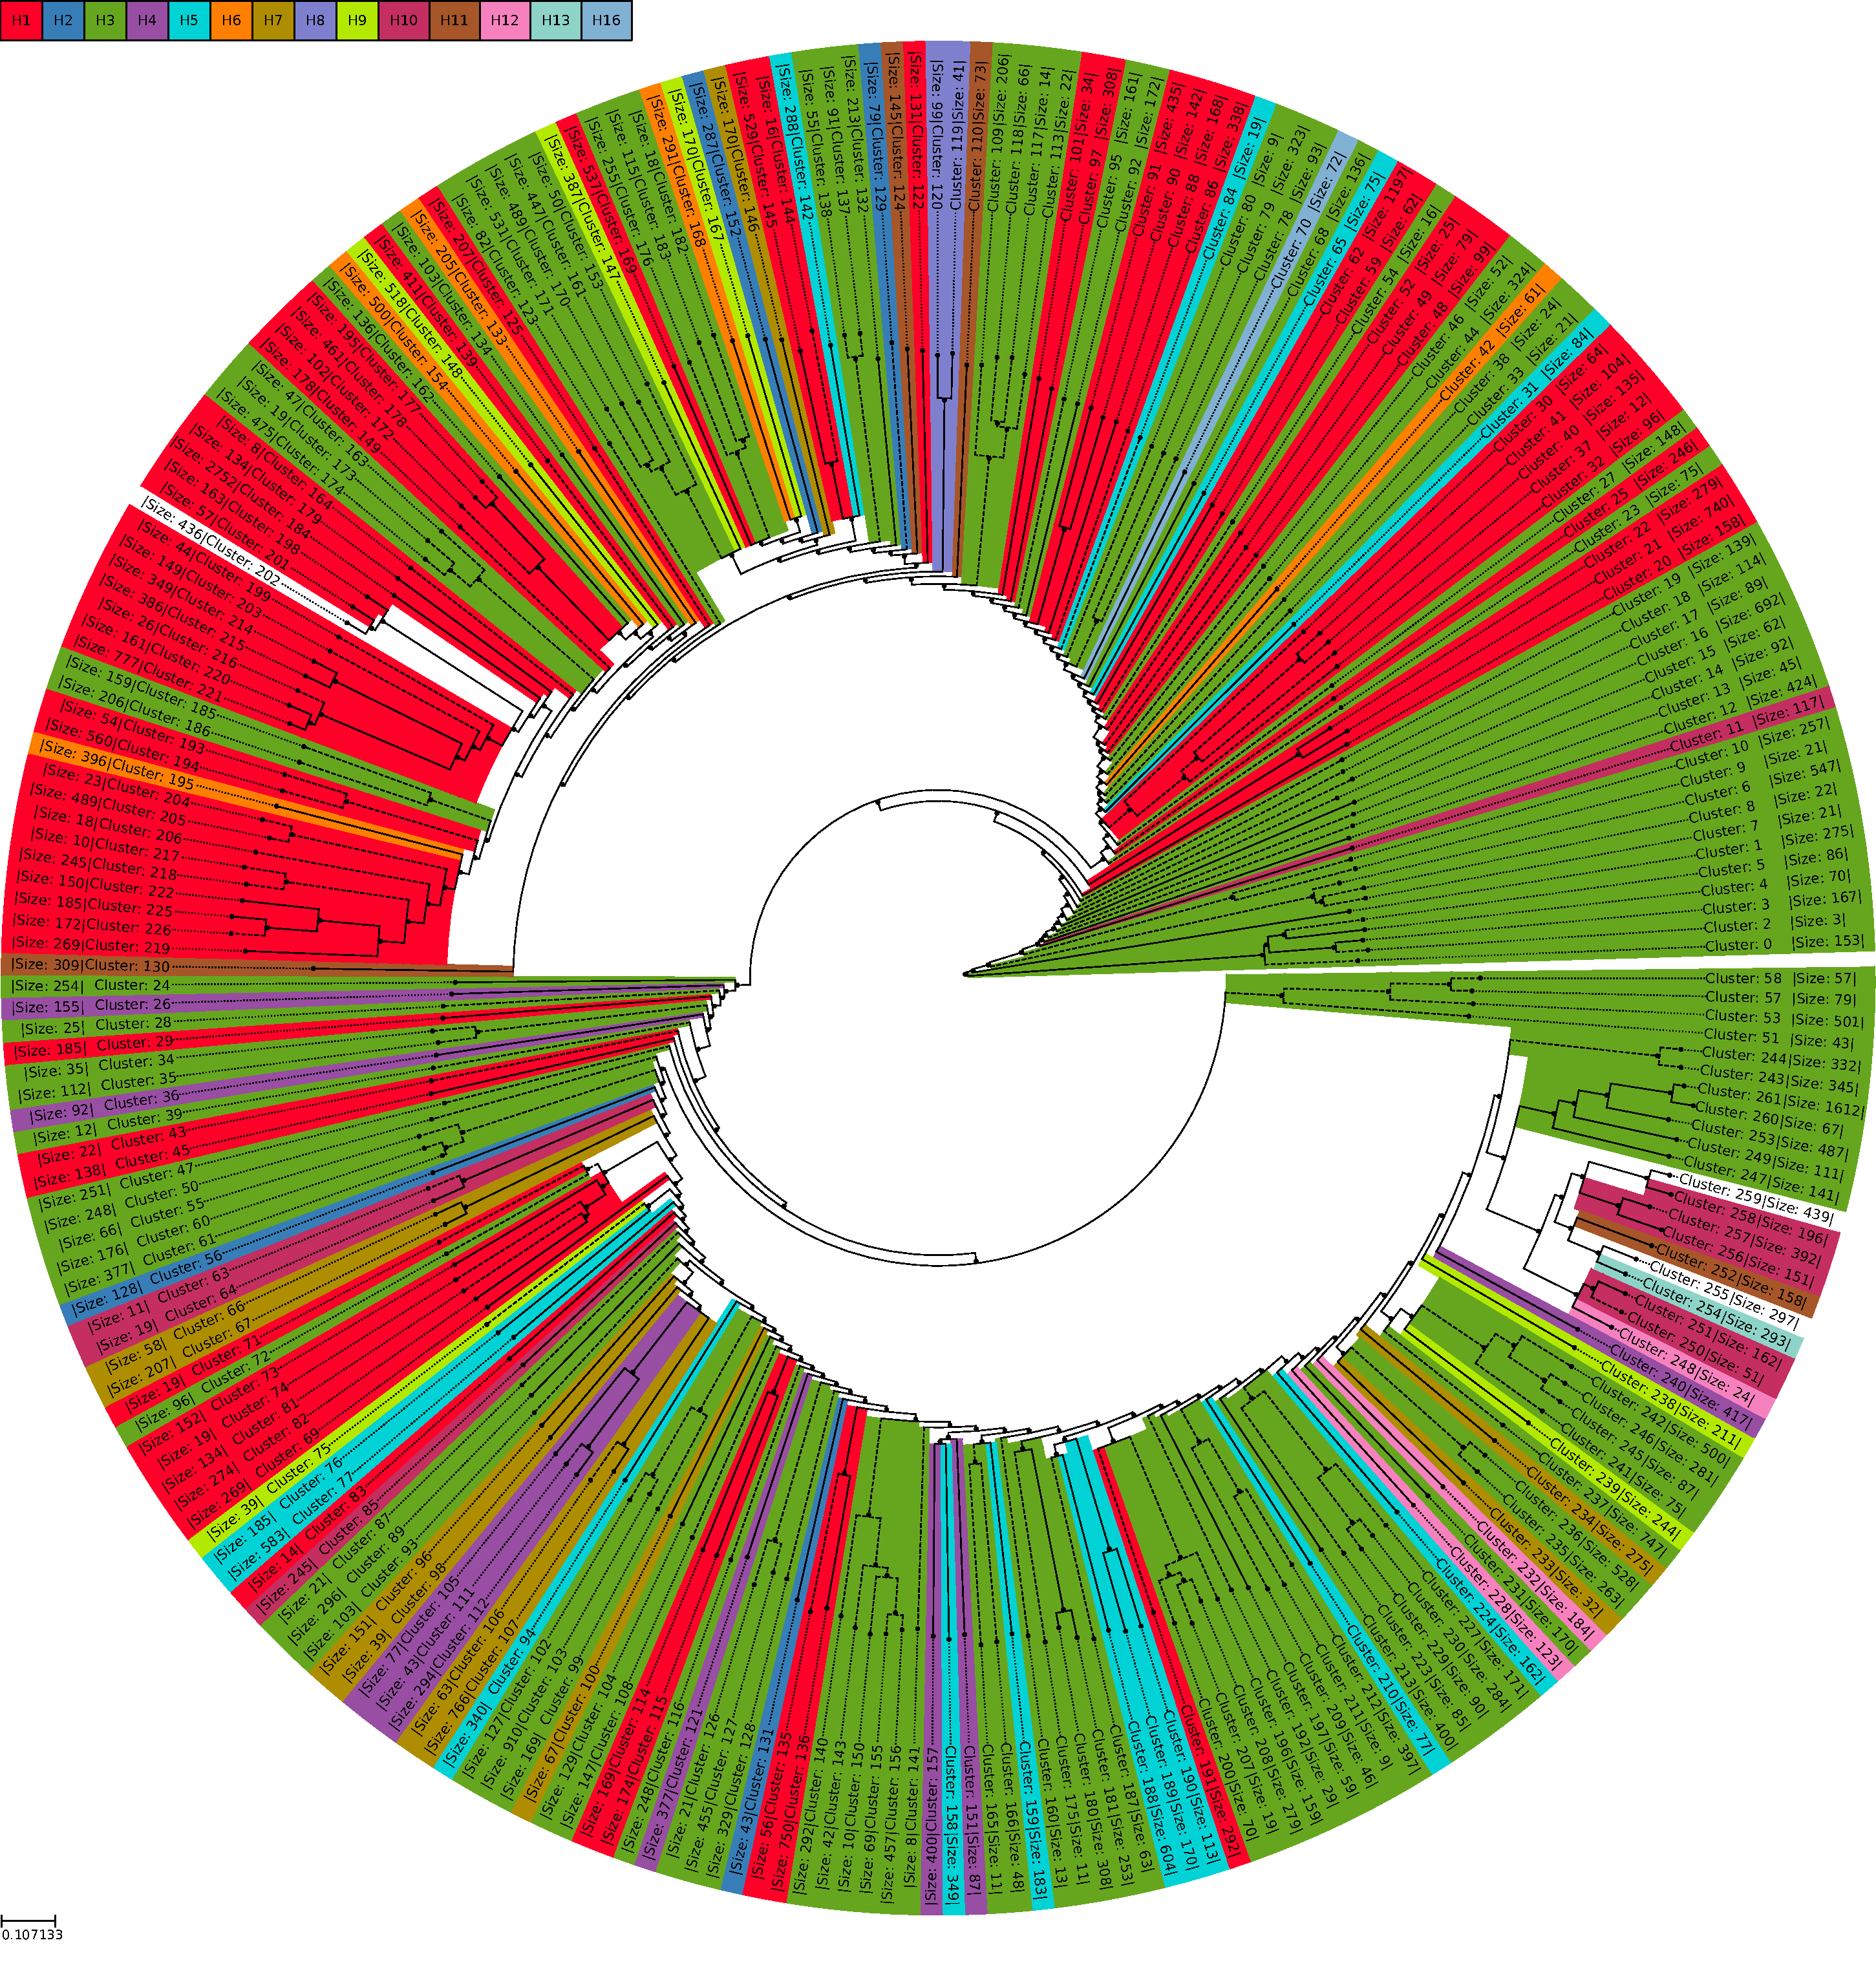
\includegraphics[width=\textwidth]{UMAP/Clustertree_Segment_4_H_Knee.pdf}
    \caption[Knee based Segment 4 Clustertree (\Acrshort{UMAP})]{\textbf{Knee based Segment 4 Clustertree (\Acrshort{UMAP}).} .}
    \label{fig:UMAP_Clusteree_Knee_4}
\end{figure}

\begin{table}[!hbt]
    \centering
    \caption[Anomalies in Segment 4 Cluster 105 (\Acrshort{UMAP})]{\textbf{Anomalies in Segment 4 Cluster 105 (\Acrshort{UMAP}).}.}
    \label{tab:UMAP_Error_4_105}
    \pgfplotstabletypeset[
        every head row/.style={
            before row={
                \toprule
            },
            after row={
                \midrule
            },
        },
        every last row/.style={
            after row={
                \bottomrule
            },
        },
        begin table=\begin{tabular*}{0.75\textwidth},
        end table=\end{tabular*},
        columns={0,1,2},
        columns/0/.style={string type,multicolumn names=l,column name=\textbf{Accession}, column type=@{\extracolsep{\fill}\hspace{6pt}}r},
        columns/1/.style={multicolumn names=l,column name=\textbf{H1}, column type=r},
        columns/2/.style={multicolumn names=l,column name=\textbf{H10}, column type=r},
    ]
    {UMAP/error_segment_4_cluster_105_difference_head.csv}
\end{table}

\begin{table}[!hbt]
    \centering
    \caption[Anomalies in Segment 4 Cluster 265 (\Acrshort{UMAP})]{\textbf{Anomalies in Segment 4 Cluster 265 (\Acrshort{UMAP}).}.}
    \label{tab:UMAP_Error_4_265}
    \pgfplotstabletypeset[
        every head row/.style={
            before row={
                \toprule
            },
            after row={
                \midrule
            },
        },
        every last row/.style={
            after row={
                ... & ... & ... & ...\\
                \bottomrule
            },
        },
        begin table=\begin{tabular*}{0.75\textwidth},
        end table=\end{tabular*},
        columns={0,1,2,3},
        columns/0/.style={string type,multicolumn names=l,column name=\textbf{Accession}, column type=@{\extracolsep{\fill}\hspace{6pt}}r},
        columns/1/.style={multicolumn names=l,column name=\textbf{H7}, column type=r},
        columns/2/.style={multicolumn names=l,column name=\textbf{H10}, column type=r},
        columns/3/.style={multicolumn names=l,column name=\textbf{H12}, column type=r},
    ]
    {UMAP/error_segment_4_cluster_265_difference_head.csv}
\end{table}

\begin{figure}[!hbt]
    \centering
    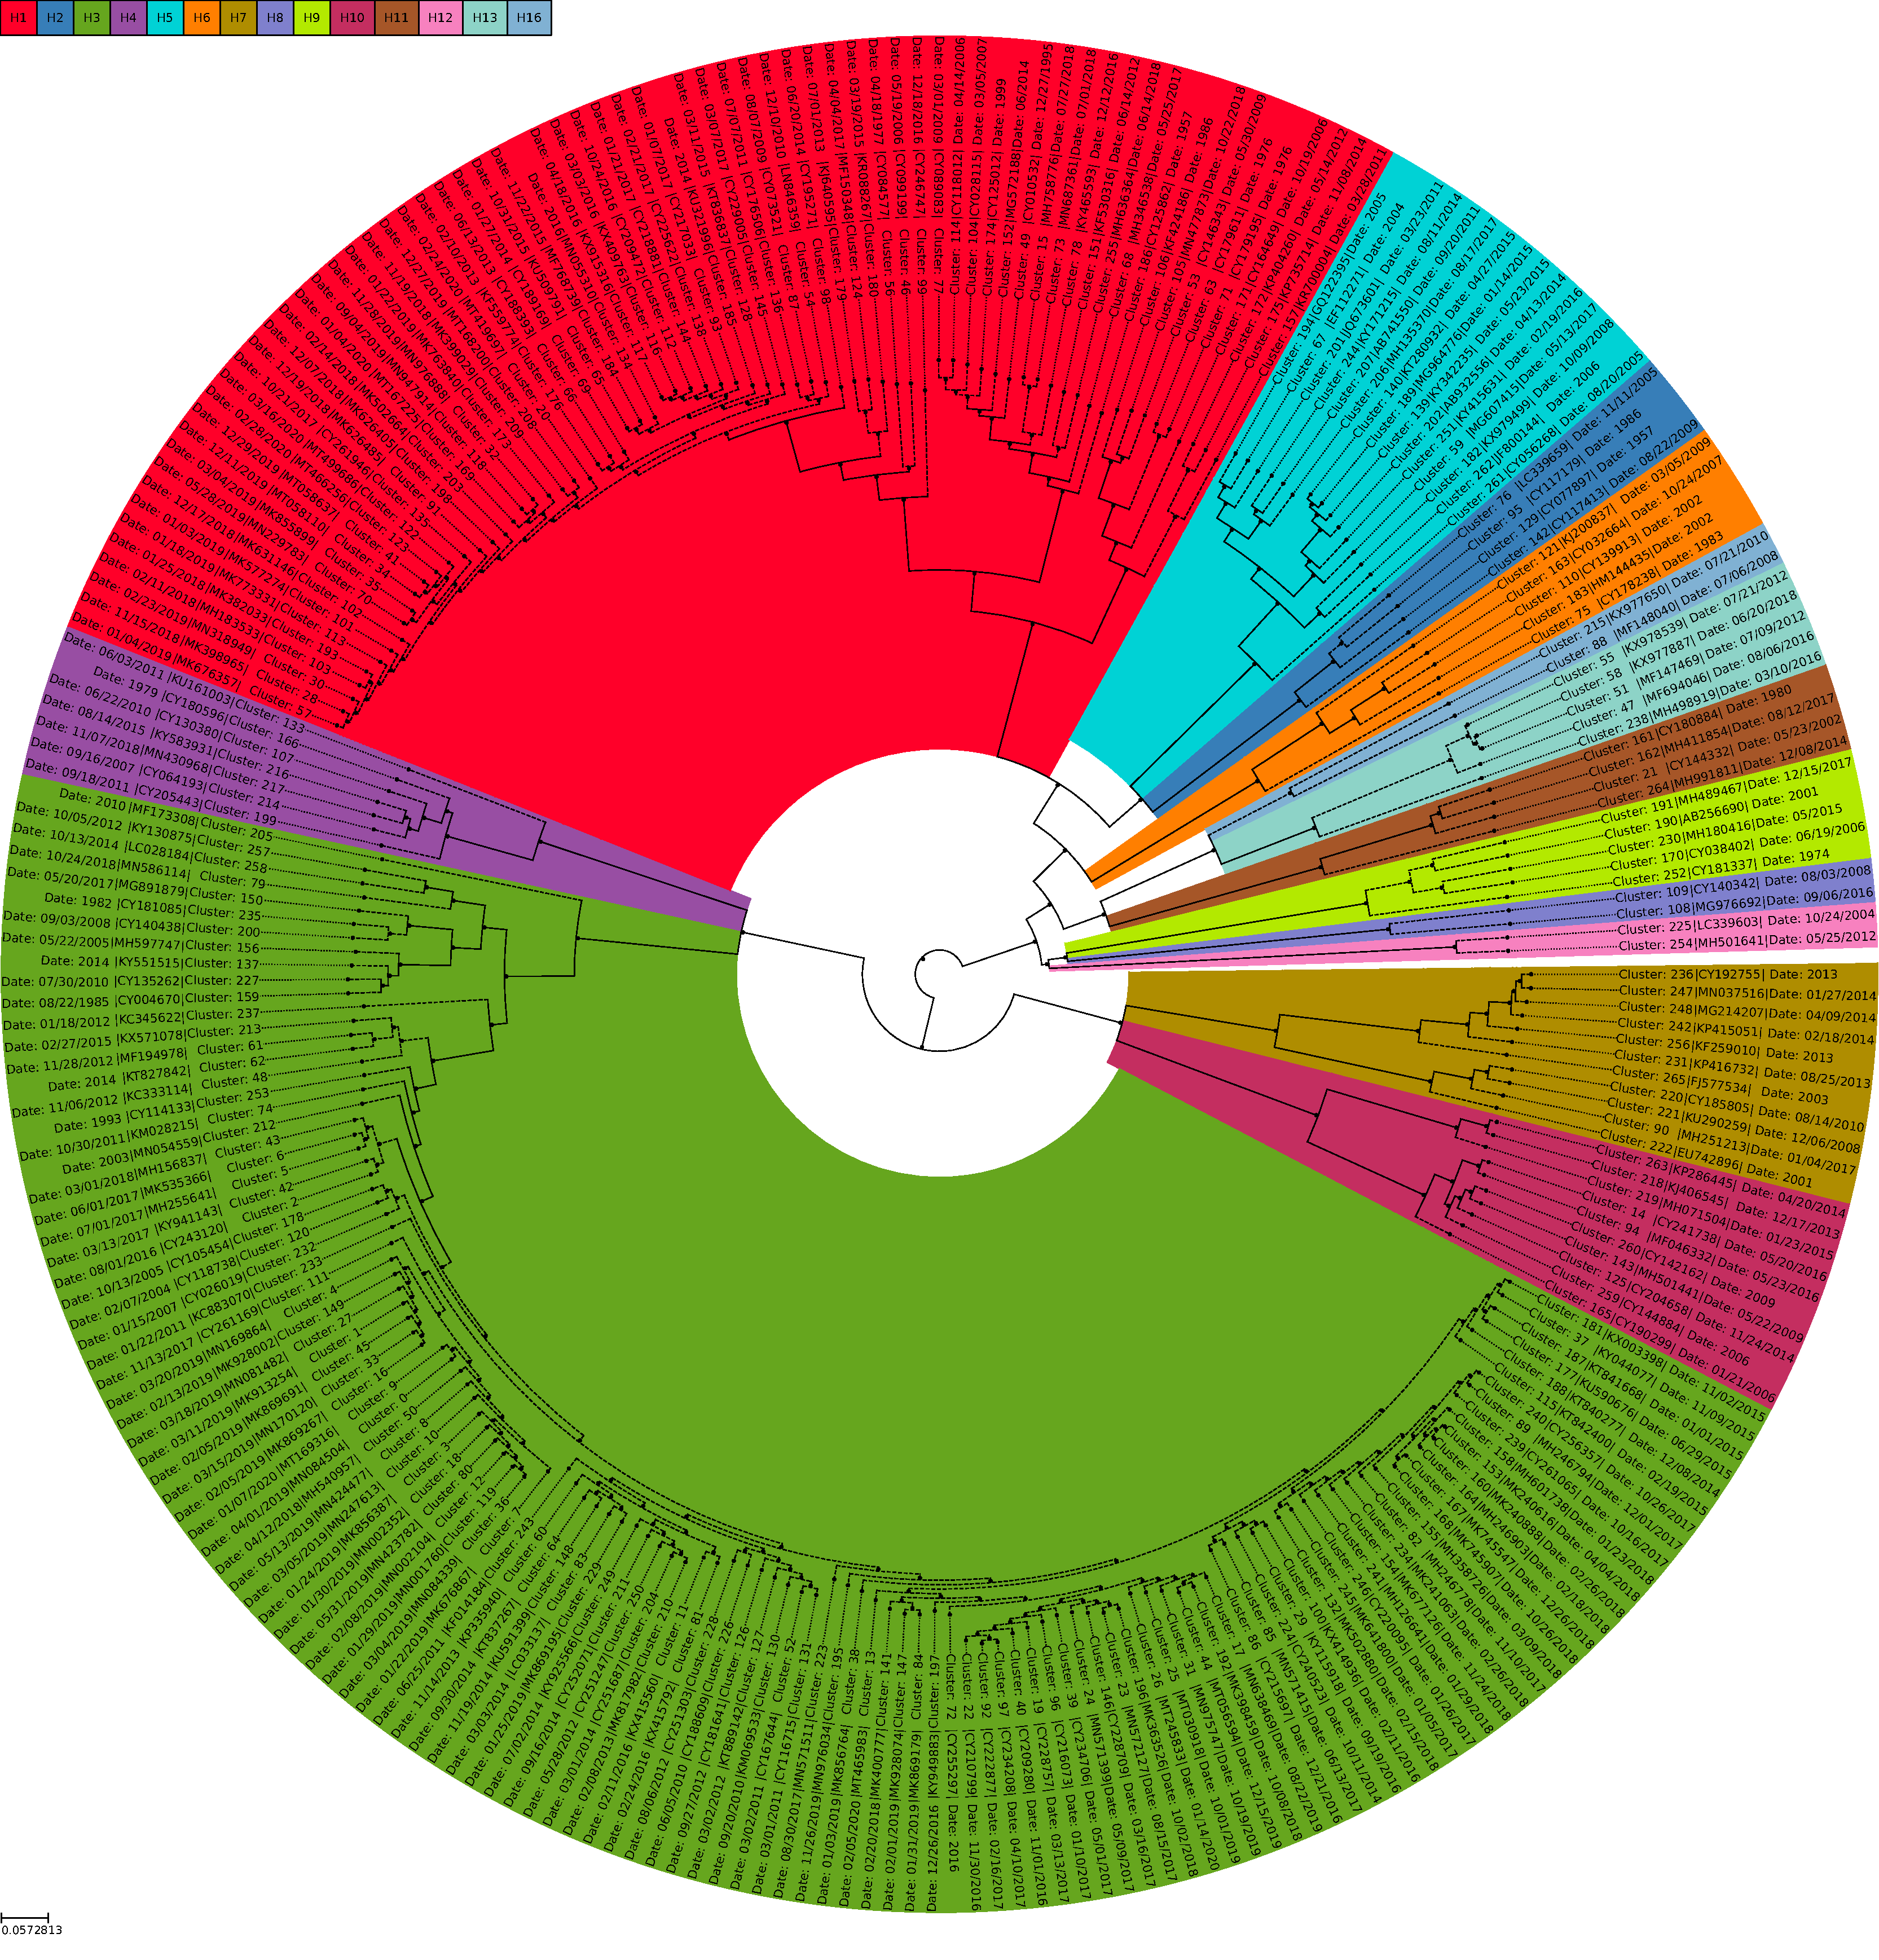
\includegraphics[width=\textwidth]{UMAP/Guidetree_segment_4_H_Centroid.pdf}
    \caption[Knee based Segment 4 Centroid Guidetree (\Acrshort{UMAP})]{\textbf{Knee based Segment 4 Centroid Guidetree (\Acrshort{UMAP}).} .}
    \label{fig:UMAP_Guidetree_Centroid_4}
\end{figure}

\begin{figure}[!hbt]
    \centering
    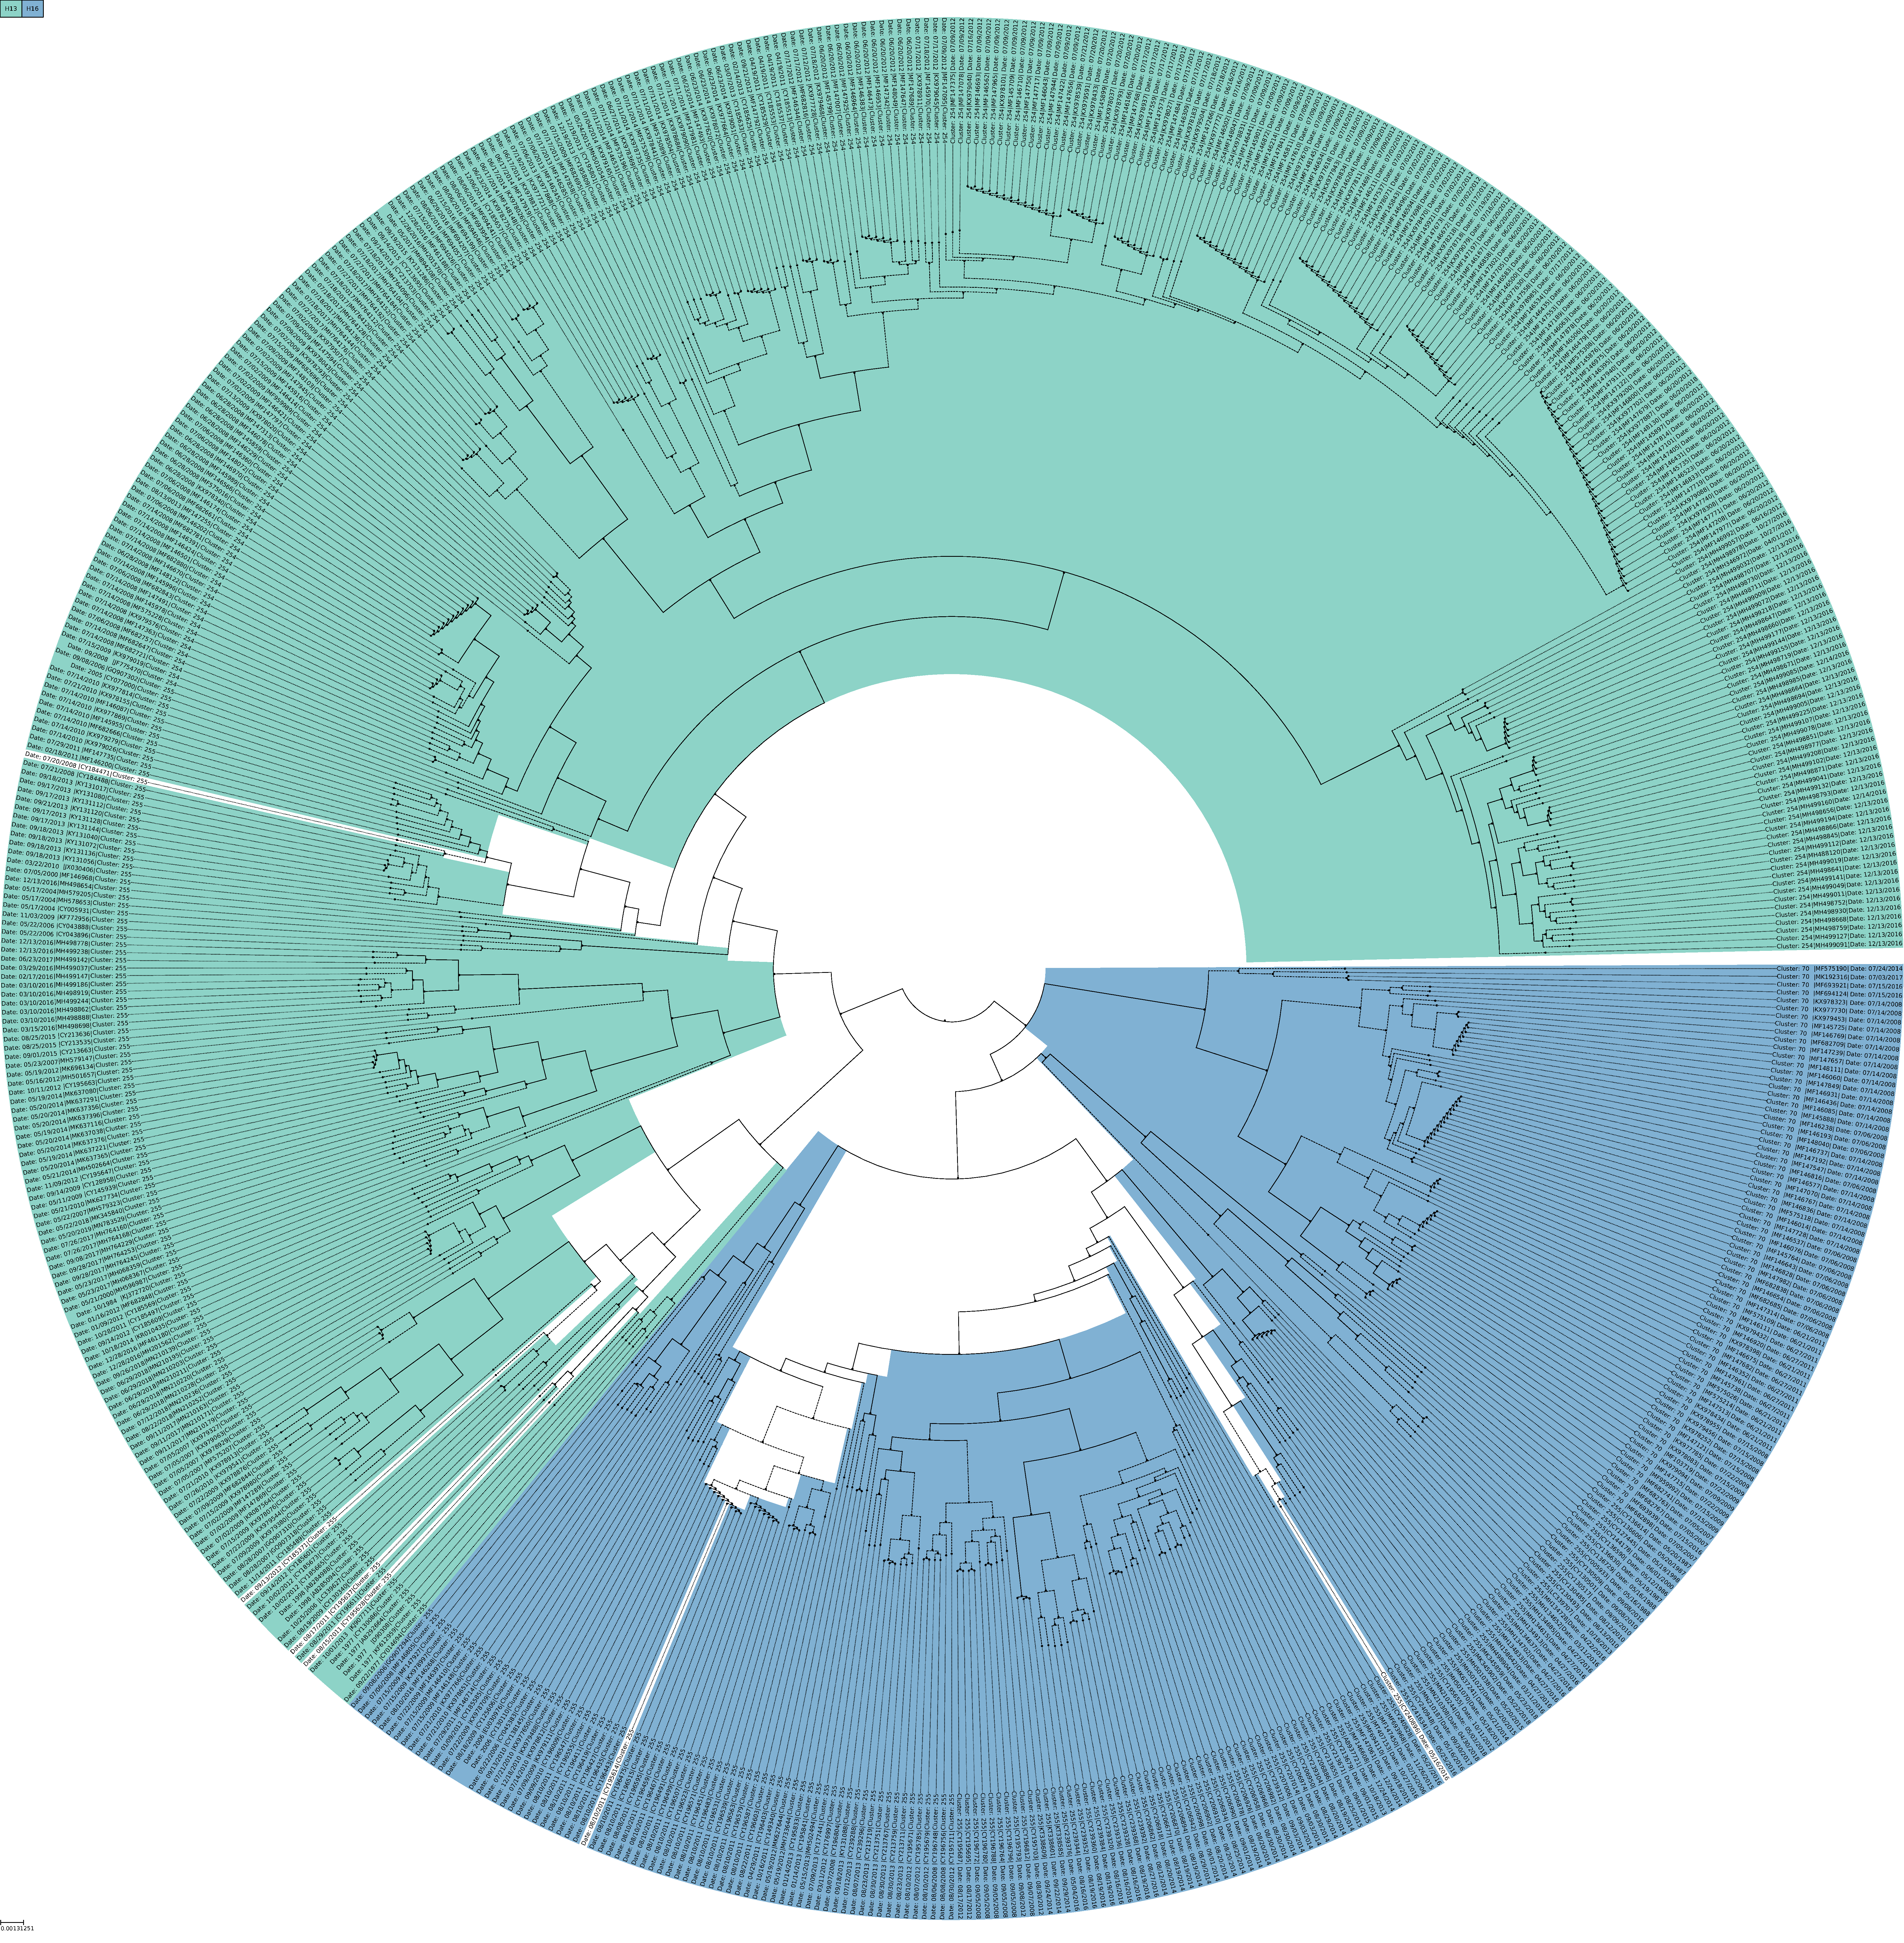
\includegraphics[width=\textwidth]{UMAP/Precalculated_Segment_4_H_Euclidean.pdf}
    \caption[H13/H16 Precalculated \Acrshort{UPGMA} Tree (euclidean)]{\textbf{H13/H16 Precalculated \Acrshort{UPGMA} Tree (euclidean).} .}
    \label{fig:Precalculated_Euclid}
\end{figure}

\begin{figure}[!hbt]
    \centering
    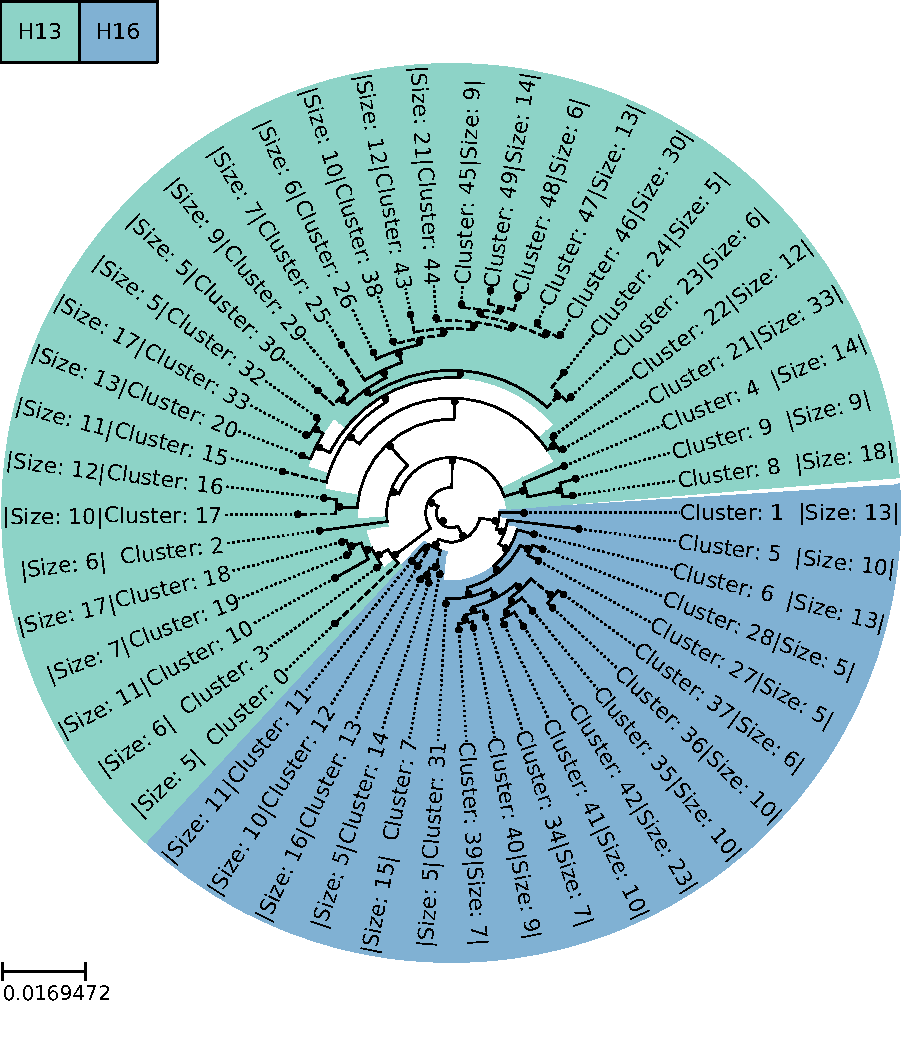
\includegraphics[width=\textwidth]{PCA/Clustertree_Segment_4_H_Euclidean.pdf}
    \caption[H13/H16 Simple Clustering Example with Precalculated (euclidean)]{\textbf{H13/H16 Simple Clustering Example with Precalculated (euclidean).} .}
    \label{fig:Simple_Clustertree_Euclid}
\end{figure}